\documentclass{article}
\usepackage{graphicx} % Required for inserting images
\usepackage{float}

\title{ECE148: Signal Processing Applications \\ \large
        Assignment 6: Signal Interpolation (FFT Applications)}
\author{Andy Chen}
\date{May 2026}

\begin{document}

\maketitle

\section{Introduction}
Consider a real and periodic signal \(f(t)\), of period \(T\). The signal has 7 harmonics, for \(m = 1, 2, ..., 7\).
\[
f(t) = \sum_{m=1}^{7} a_m \sin\bigg(\frac{2m\pi t}{T}\bigg)
\]
The seven coefficients \(\{a_m\}\) are formed with my personal 7-digit UCSB perm number (1055388). A discrete sequence can be formed by taking N uniform samples within one period with sample spacing \(\Delta t = \frac{T}{N}\). For this assignment, we produce three sequences, \(f(n)\),  \(g(n)\), and \(p(n)\), by sampling \(f(t)\) at different rates, for \(N=16\), 64, and 256 respectively.

\section{Plotting the Sequences \(f(n), \ g(n),\) and \(p(n)\)}
For each value of \(N\), the sampling interval is \(\Delta t = \frac{T}{N}\), with samples occurring at \(n\Delta t\), where \(n = 0, 1, 2,...,N-1\). Thus, for \(N=16\), we expect coarse sampling, \(N=64\), we expect improved resolution, and \(N=256\), we expect a very fine approximation to the continuous waveform.
\begin{figure}[H]
    \centering
    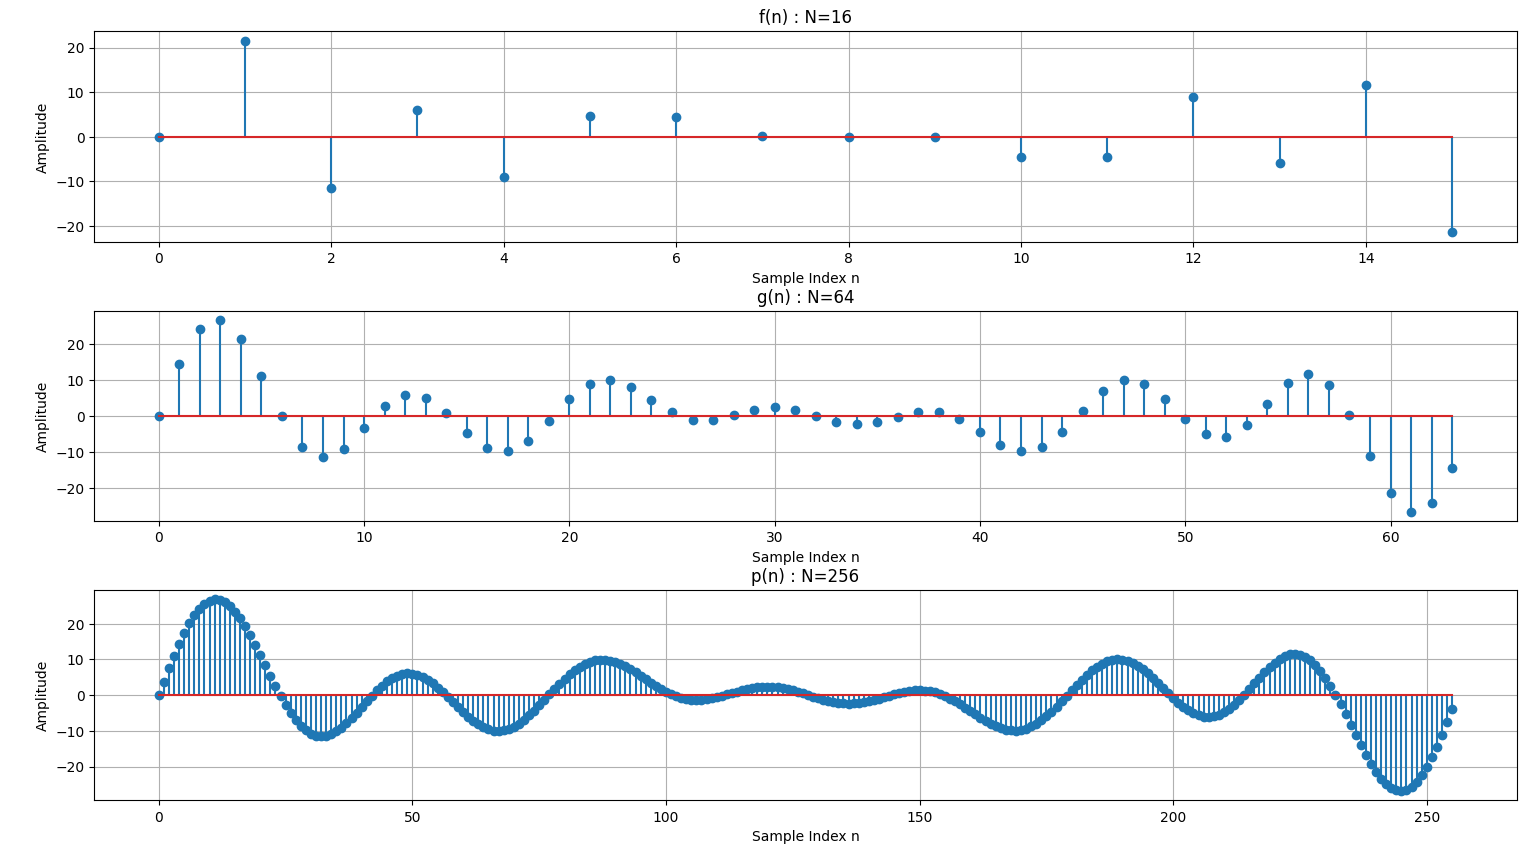
\includegraphics[width=1\linewidth]{sequence_plotting.png}
    \caption{From top to bottom: the plot of \(f(n)\), the plot of \(g(n)\), and the plot of \(p(n)\).}
    \label{fig:placeholder}
\end{figure}

\section{FFT Interpolation from 16 to 64 Samples}
We take the 16-point DFT of \(f(n)\):
\[
F(k) = \sum_{n=0}^{15} f(n) e^{-j2\pi kn/16}
\]
to convert the sequence into the frequency domain. To interpolate in time, we insert zeros into the FFT spectrum. Increasing the FFT length from 16 to 64 effectively increases the number of time-domain samples after the inverse FFT. After zero padding and after taking the inverse FFT, a scaling factor \(\frac{64}{16}=4\) is required because FFT implementations distribute scaling differently between FFT and inverse FFT.
\begin{figure}[H]
    \centering
    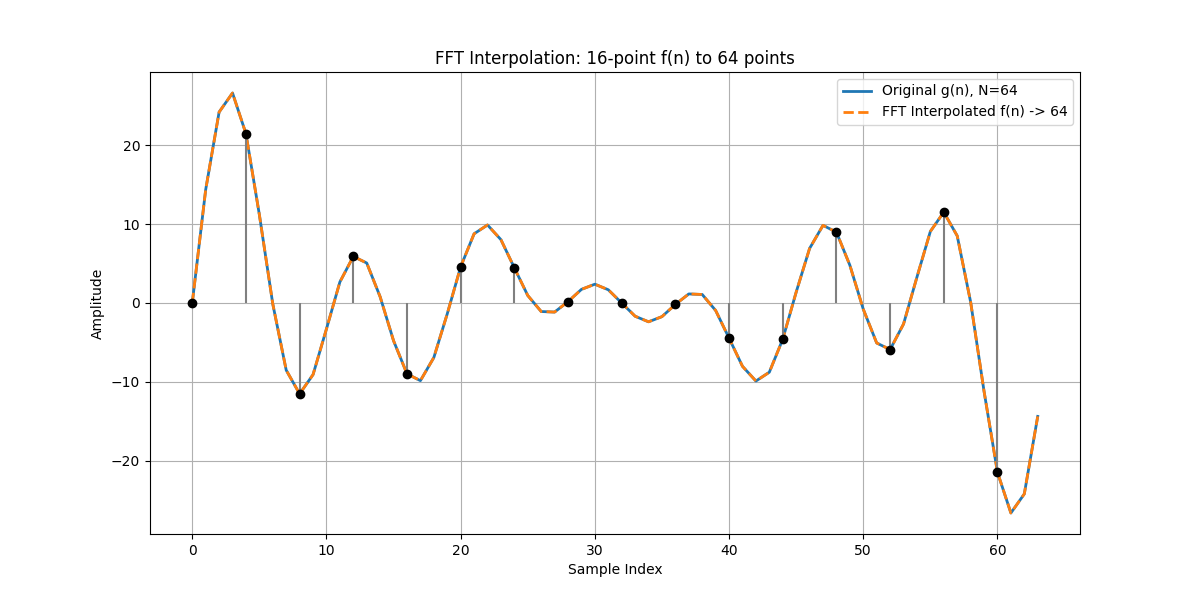
\includegraphics[width=1\linewidth]{fft_interpolation1664.png}
    \caption{FFT interpolation from 16 to 64 samples.}
    \label{fig:placeholder}
\end{figure}
The interpolated sequence closely matches \(g(n)\). Because the original signal contains only 7 harmonics, the 16-point sampling rate satisfies Nyquist: \[N=16 > 2 \times 7 = 14\] No aliasing occurs, the spectrum is fully recoverable, and FFT interpolation reconstructs the intermediate samples accurately.

\section{FFT Interpolation from 16 to 256 Samples}
To interpolate the 16-point sequence \(f(n)\) to 256 points using FFT, we again use frequency-domain zero padding. After taking the inverse FFT, we apply a scaling factor of \(\frac{256}{16} = 16\) to correct the amplitude after interpolation.
\begin{figure}[H]
    \centering
    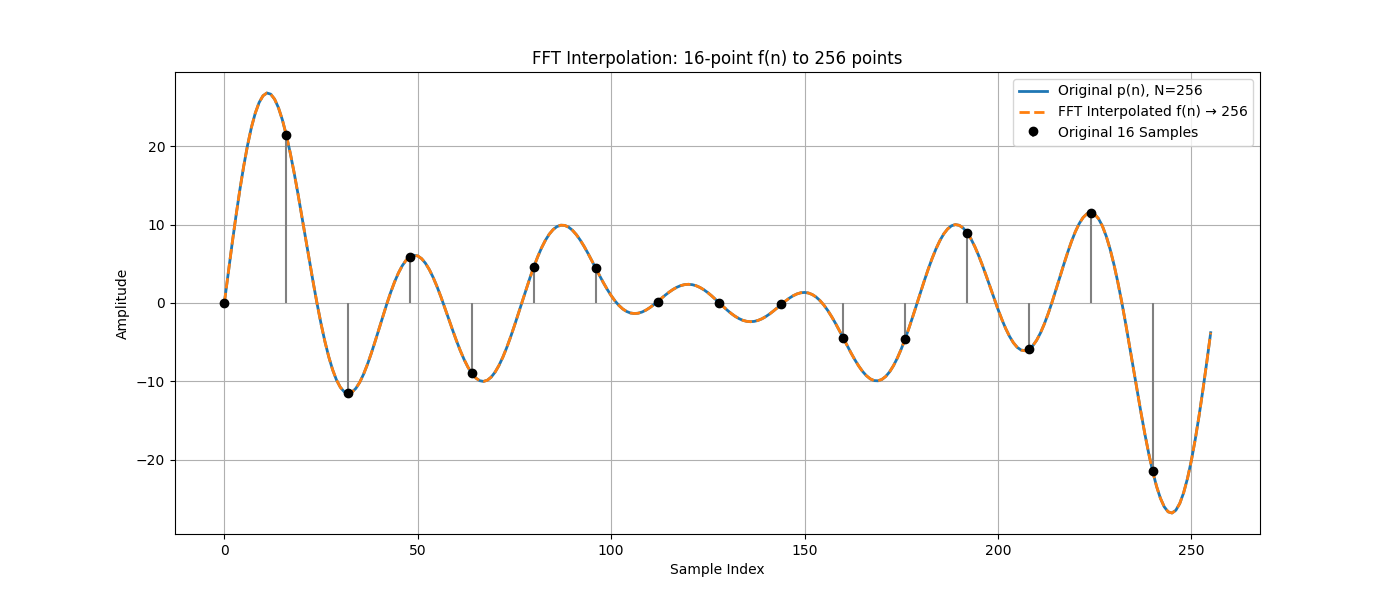
\includegraphics[width=1\linewidth]{fft_interpolation16256.png}
    \caption{FFT interpolation from 16 to 256 samples.}
    \label{fig:placeholder}
\end{figure}
The interpolated sequence closely matches \(p(n)\), and is smoother than the previous interpolated sequence. Because the original sequence was sampled above the Nyquist rate, the signal is fully recoverable, and FFT interpolation reproduces the higher-resolution sampled sequences accurately. 

\section{What if the number of data samples is not a power of 2?}
The FFT algorithm is most efficient when the number of samples \(N\) is a power of two: \(N= 2^k\) because the standard FFT algorithm repeatedly divides the DFT into smaller halves. This gives a time complexity of \(O(N \log_2 N)\). 
\\
\\When \(N\) is not a power of two, this recursive division fails, resulting in a slower calculation. Essentially, the algorithm is optimized for calculations for sample sizes that are powers of two. Because of this, we must zero-pad to the next power of two for optimal FFT computation.

\section{What if the FFT spectral data at \(k=\frac{N}{2}\) is nonzero?}
For an even-length FFT, the spectral index \(k=\frac{N}{2}\) corresponds to the Nyquist frequency \(\frac{f_s}{2}\). For real-valued signals, the DC bin is purely real, and the Nyquist bin is also purely real. This occurs because the Nyquist frequency is its own negative-frequency pair, so it does not form a conjugate pair with another bin. 
\\
\\
If the Nyquist bin is nonzero, you cannot zero pad without breaking symmetry or creating interpolation artifacts. The Nyquist component must be split evenly between the positive and negative sides after padding to preserve Hermitian symmetry. If the bin is not split, the resulting interpolated signal will become complex-valued rather than remaining strictly real.

\section{2D FFT Interpolation (\(16\times16 \rightarrow 64\times 64\))}
We consider an array of \(16 \times 16\) data samples. For a 2D signal, interpolation using the FFT is performed by zero-padding the spectrum in the frequency domain, then applying the inverse FFT.
\\
\\
Given the original sampled data:
\[
f(m,n), \qquad 0\leq m, n\leq 15
\]
The desired interpolated array:
\[
g(m,n), \qquad 0\leq m, n\leq 63 
\]
And a scaling factor \(\frac{64}{16}=4\) in both dimensions.

\subsection*{1. Compute the 2D FFT}
We take the 2D FFT of the \(16 \times 16\) array:
\[
F(k,l) = \sum_{m=0}^{15} \sum_{n=0}^{15} f(m,n)e^{-j2\pi(\frac{km}{16} + \frac{ln}{16})}
\]
This converts the spatial-domain data into the 2D frequency domain.

\subsection*{2. Shift the Spectrum to the Center}
We shift the zero-frequency component to the frequency. This rearranges the spectrum so that low frequencies are centered and high frequencies move toward the edges.

\subsection*{3. Zero-Padding the Spectrum}
We create a \(64 \times 64\) array filled with zeros, where we embed the centered \(16\times 16\) spectrum into the middle. Essentially, we have zeros surrounding the original spectrum, padding it out to size \(64 \times 64\).

\subsection*{4. Shift Back}
We undo the FFT shift to arrange the spectrum correctly for the inverse FFT.

\subsection*{5. Compute the Inverse 2D FFT}
We apply the inverse 2D FFT and reconstruct the interpolated spatial-domain data.

\subsection*{6. Scale the Result}
Because the array size increased, the result must be scaled by:
\[
\bigg(\frac{64}{16}\bigg)^2
\]
We square the scaling factor because interpolation occurs in both dimensions.
The result is a smooth, high-resolution reconstruction of the original 2D sampled data.
\begin{figure}
    \centering
    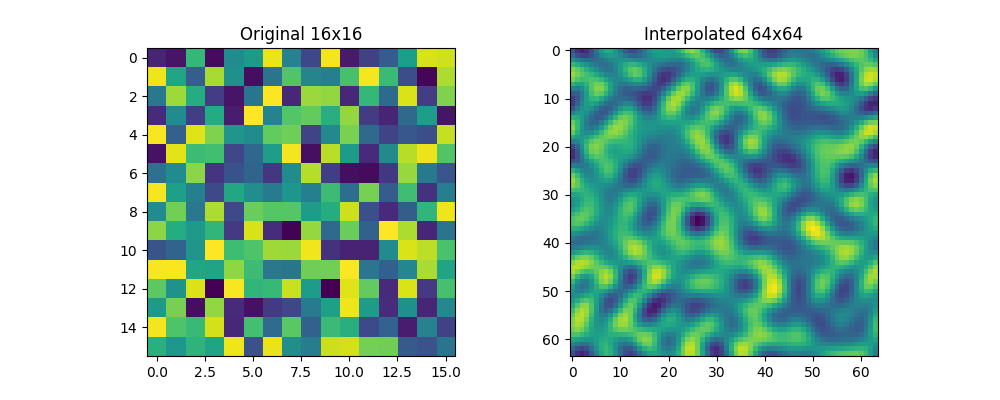
\includegraphics[width=1\linewidth]{2dfft_interpolation.png}
    \caption{An example of the 2D FFT interpolation procedure.}
    \label{fig:placeholder}
\end{figure}

\end{document}
